% Options for packages loaded elsewhere
\PassOptionsToPackage{unicode}{hyperref}
\PassOptionsToPackage{hyphens}{url}
%
\documentclass[
  ignorenonframetext,
]{beamer}
\usepackage{pgfpages}
\setbeamertemplate{caption}[numbered]
\setbeamertemplate{caption label separator}{: }
\setbeamercolor{caption name}{fg=normal text.fg}
\beamertemplatenavigationsymbolsempty
% Prevent slide breaks in the middle of a paragraph
\widowpenalties 1 10000
\raggedbottom
\setbeamertemplate{part page}{
  \centering
  \begin{beamercolorbox}[sep=16pt,center]{part title}
    \usebeamerfont{part title}\insertpart\par
  \end{beamercolorbox}
}
\setbeamertemplate{section page}{
  \centering
  \begin{beamercolorbox}[sep=12pt,center]{part title}
    \usebeamerfont{section title}\insertsection\par
  \end{beamercolorbox}
}
\setbeamertemplate{subsection page}{
  \centering
  \begin{beamercolorbox}[sep=8pt,center]{part title}
    \usebeamerfont{subsection title}\insertsubsection\par
  \end{beamercolorbox}
}
\AtBeginPart{
  \frame{\partpage}
}
\AtBeginSection{
  \ifbibliography
  \else
    \frame{\sectionpage}
  \fi
}
\AtBeginSubsection{
  \frame{\subsectionpage}
}
\usepackage{amsmath,amssymb}
\usepackage{iftex}
\ifPDFTeX
  \usepackage[T1]{fontenc}
  \usepackage[utf8]{inputenc}
  \usepackage{textcomp} % provide euro and other symbols
\else % if luatex or xetex
  \usepackage{unicode-math} % this also loads fontspec
  \defaultfontfeatures{Scale=MatchLowercase}
  \defaultfontfeatures[\rmfamily]{Ligatures=TeX,Scale=1}
\fi
\usepackage{lmodern}
\usetheme[]{metropolis}
\ifPDFTeX\else
  % xetex/luatex font selection
\fi
% Use upquote if available, for straight quotes in verbatim environments
\IfFileExists{upquote.sty}{\usepackage{upquote}}{}
\IfFileExists{microtype.sty}{% use microtype if available
  \usepackage[]{microtype}
  \UseMicrotypeSet[protrusion]{basicmath} % disable protrusion for tt fonts
}{}
\makeatletter
\@ifundefined{KOMAClassName}{% if non-KOMA class
  \IfFileExists{parskip.sty}{%
    \usepackage{parskip}
  }{% else
    \setlength{\parindent}{0pt}
    \setlength{\parskip}{6pt plus 2pt minus 1pt}}
}{% if KOMA class
  \KOMAoptions{parskip=half}}
\makeatother
\usepackage{xcolor}
\newif\ifbibliography
\usepackage{graphicx}
\makeatletter
\def\maxwidth{\ifdim\Gin@nat@width>\linewidth\linewidth\else\Gin@nat@width\fi}
\def\maxheight{\ifdim\Gin@nat@height>\textheight\textheight\else\Gin@nat@height\fi}
\makeatother
% Scale images if necessary, so that they will not overflow the page
% margins by default, and it is still possible to overwrite the defaults
% using explicit options in \includegraphics[width, height, ...]{}
\setkeys{Gin}{width=\maxwidth,height=\maxheight,keepaspectratio}
% Set default figure placement to htbp
\makeatletter
\def\fps@figure{htbp}
\makeatother
\setlength{\emergencystretch}{3em} % prevent overfull lines
\providecommand{\tightlist}{%
  \setlength{\itemsep}{0pt}\setlength{\parskip}{0pt}}
\setcounter{secnumdepth}{-\maxdimen} % remove section numbering
\usepackage{luatexja}
\usepackage{luatexja-fontspec}

% for video embedding
\usepackage{multimedia}
% Show speaker note
\mode<beamer>{
  \setbeameroption{show notes on second screen}
  \setbeamertemplate{note page}[plain]
}
\ifLuaTeX
  \usepackage{selnolig}  % disable illegal ligatures
\fi
\IfFileExists{bookmark.sty}{\usepackage{bookmark}}{\usepackage{hyperref}}
\IfFileExists{xurl.sty}{\usepackage{xurl}}{} % add URL line breaks if available
\urlstyle{same}
\hypersetup{
  pdftitle={Pandoc beamer sample},
  pdfauthor={taishi-n},
  hidelinks,
  pdfcreator={LaTeX via pandoc}}

\title{Pandoc beamer sample}
\subtitle{with pympress}
\author{taishi-n}
\date{\today}
\institute{qiita}

\begin{document}
\frame{\titlepage}

\subsection{基本的な使い方}\label{ux57faux672cux7684ux306aux4f7fux3044ux65b9}

\begin{frame}{数式}
\phantomsection\label{ux6570ux5f0f}
\metroset{block=fill}

\begin{block}{Fourier Transform}
\phantomsection\label{fourier-transform}
\[X(\omega) = \int _{-\infty} ^{\infty} x(t) \exp \left(- j{2\pi f t}\right) \mathrm{d}t\]
\[x(t) = \int _{-\infty} ^{\infty} X(\omega) \exp \left( j{2\pi f t}\right) \mathrm{d}\omega\]
\end{block}

\begin{block}{Discrete Fourier Transform}
\phantomsection\label{discrete-fourier-transform}
\[X_k = \sum _{n=0} ^{N-1} x_n \exp \left(- j\frac{2\pi n k}{N} \right)\]
\[x_n = \sum _{k=0} ^{N-1} x_n \exp \left(+ j\frac{2\pi n k}{N} \right)\]
\end{block}
\end{frame}

\begin{frame}{画像の挿入}
\phantomsection\label{ux753bux50cfux306eux633fux5165}
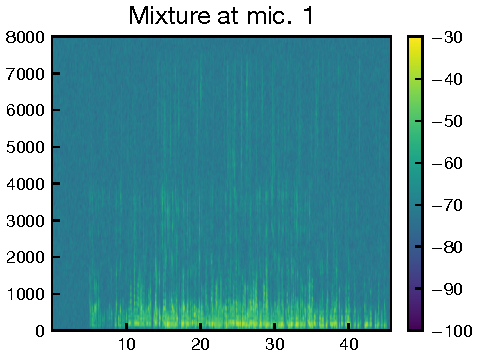
\includegraphics{spec.pdf}
\end{frame}

\subsection{応用編}\label{ux5fdcux7528ux7de8}

\begin{frame}{カラム分割}
\phantomsection\label{ux30abux30e9ux30e0ux5206ux5272}
\begin{columns}[T]
\begin{column}{0.4\textwidth}
\begin{itemize}
\tightlist
\item
  列に分割して何かを並べたい時に重宝します
\item
  この例では左側 40\%右側 60\%としています
\end{itemize}
\end{column}

\begin{column}{0.6\textwidth}
\begin{itemize}
\tightlist
\item
  もちろん画像や数式の挿入もできます
\end{itemize}

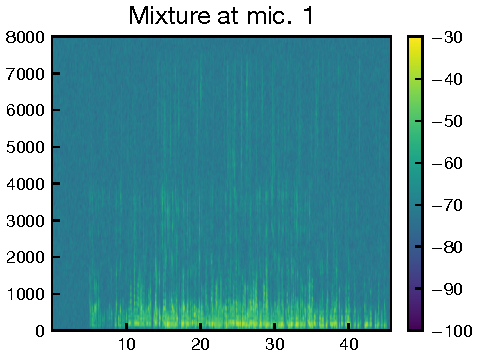
\includegraphics{spec.pdf}

\[X_k = \sum _{n=0} ^{N-1} x_n \exp \left(- j\frac{2\pi n k}{N} \right)\]
\end{column}
\end{columns}
\end{frame}

\begin{frame}{TeX コードの直接入力}
\phantomsection\label{tex-ux30b3ux30fcux30c9ux306eux76f4ux63a5ux5165ux529b}
\begin{itemize}
\tightlist
\item
  どうしても markdown で無理があるという場合は TeX
  コードを直接打ち込むこともできます
\end{itemize}

\begin{figure}[t]
\centering
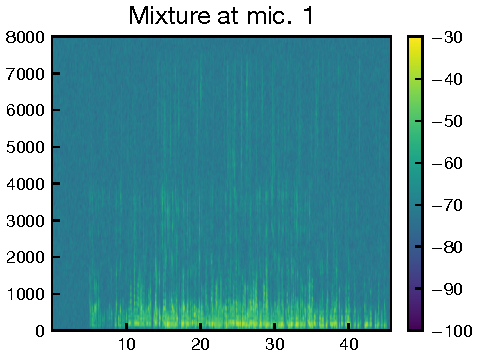
\includegraphics[height=.5\textwidth]{spec.pdf}
\end{figure}
\end{frame}

\begin{frame}[fragile]{note 機能}
\phantomsection\label{note-ux6a5fux80fd}
\begin{itemize}
\item
  スピーカーノート
\item
  プリアンブルに下記を追加

\begin{verbatim}
\mode<beamer>{
  \setbeameroption{show notes on second screen}
  \setbeamertemplate{note page}[plain]
}
\end{verbatim}
\item
  \href{https://github.com/Cimbali/pympress}{pympress}と連携可能
\end{itemize}

\note{\begin{itemize}
\tightlist
\item
  いわゆるスピーカーノートです
\item
  プリアンブルに次のような命令を書くことで左側にスライド本体,右側に台本が表示された横長の
  pdf が生成されます
\item
  pympress で生成された pdf
  を開いて,スピーカーノートが右側にあることを設定で与えるとパワポの発表者画面のようになります
\item
  時間管理もできてなにげに便利です
\end{itemize}}
\end{frame}

\begin{frame}{動画の再生}
\phantomsection\label{ux52d5ux753bux306eux518dux751f}
\begin{itemize}
\item
  pympress を使えば動画も再生可能

  \movie[height=18pt]{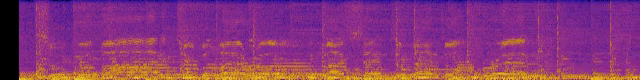
\includegraphics[height=18pt]{mix.png}}{mix.mp4}
\end{itemize}
\end{frame}

\end{document}
